% Supplementary material for the Physiological Measurement manuscript (main.tex).
% Same rule as the main text: every number comes from numbers.tex, numbers_r3.tex or numbers_ext.tex,
% every table from tables/ and every figure from figures/, all written by paper/make_assets.py.
% Build: bash paper/build.sh (compiles main.tex and this file).
\documentclass{iopjournal}
\usepackage{amsmath}
\usepackage{graphicx}
\usepackage[round,authoryear]{natbib}
% generated by paper/make_assets.py -- do not edit
\newcommand{\nAll}{366,185}
\newcommand{\nTrain}{292,885}
\newcommand{\nTest}{73,300}
\newcommand{\nTestPos}{1,662}
\newcommand{\testPrev}{2.27}
\newcommand{\nCodeShort}{204,522}
\newcommand{\nCodeLong}{131,734}
\newcommand{\nCodeShortPos}{6,236}
\newcommand{\nCodeLongPos}{317}
\newcommand{\nCodePos}{6,559}
\newcommand{\prevShort}{3.05}
\newcommand{\prevLong}{0.24}
\newcommand{\prevRatio}{12.7}
\newcommand{\shareCodePosShort}{95.1}
\newcommand{\shareAllShort}{56}
\newcommand{\nSsevenPos}{1,259}
\newcommand{\nStenPos}{77}
\newcommand{\nSseven}{40,867}
\newcommand{\nSten}{26,435}
\newcommand{\nStenPlusPos}{240}
\newcommand{\nStenPlusPosSami}{163}
\newcommand{\durOnlyB}{0.677}
\newcommand{\durOnlyA}{0.647}
\newcommand{\rowZeroA}{0.412}
\newcommand{\rowZeroAauc}{0.847}
\newcommand{\rowZeroSseven}{0.377}
\newcommand{\rowZeroSsevenAuc}{0.807}
\newcommand{\rowZeroGap}{$+0.30$}
\newcommand{\bzA}{0.436}
\newcommand{\bzAsd}{0.010}
\newcommand{\bzAauc}{0.829}
\newcommand{\bzBauc}{0.830}
\newcommand{\bzSseven}{0.384}
\newcommand{\bzSsevenSd}{0.017}
\newcommand{\bzSsevenAuc}{0.787}
\newcommand{\bzStenAuc}{0.695}
\newcommand{\bzStenPlusAuc}{0.779}
\newcommand{\bzEnsA}{0.452}
\newcommand{\bzEnsSseven}{0.404}
\newcommand{\bzEnsSsevenAuc}{0.801}
\newcommand{\bzGap}{$+0.17$}
\newcommand{\bzNegShort}{0.57}
\newcommand{\bzNegLong}{0.40}
\newcommand{\fullAuc}{0.791}
\newcommand{\fullA}{0.427}
\newcommand{\fullSsevenAuc}{0.751}
\newcommand{\aucInflation}{0.043}
\newcommand{\rowZeroInflA}{0.035}
\newcommand{\rowZeroInflAuc}{0.040}
\newcommand{\ladderGainA}{0.023}
\newcommand{\rowZeroInflBAuc}{0.044}
\newcommand{\rowZeroStenAuc}{0.720}
\newcommand{\seSsevenTpr}{0.013}
\newcommand{\demoDropDSseven}{$+0.021$}
\newcommand{\demoDropNse}{1.6}
\newcommand{\ptbRowFour}{0.24}
\newcommand{\ptbRowFive}{0.01}
\newcommand{\ptbRowFiveB}{0.07}
\newcommand{\ptbRowZero}{0.08}
\newcommand{\ptbRowTwo}{0.08}
\newcommand{\ptbRowThree}{0.32}
\newcommand{\rowOneGap}{$+0.30$}
\newcommand{\rowTwoGap}{$+0.16$}
\newcommand{\lrMidSseven}{0.381}
\newcommand{\lrLowSseven}{0.362}
\newcommand{\lrMidA}{0.423}
\newcommand{\lrLowA}{0.404}
\newcommand{\bestEpHigh}{1.7}
\newcommand{\bestEpMid}{2.7}
\newcommand{\bestEpLow}{6.7}
\newcommand{\mOneA}{0.401}
\newcommand{\mOneSseven}{0.382}
\newcommand{\mOneGap}{$+0.04$}
\newcommand{\mOneStenPlusAuc}{0.817}
\newcommand{\wOneA}{0.428}
\newcommand{\wOneSseven}{0.380}
\newcommand{\wOneGap}{$+0.10$}
\newcommand{\wOneSsevenAuc}{0.795}
\newcommand{\wOneStenPlusAuc}{0.835}
\newcommand{\mwA}{0.403}
\newcommand{\mwSseven}{0.375}
\newcommand{\mwSsevenSd}{0.011}
\newcommand{\mwSsevenAuc}{0.795}
\newcommand{\mwStenAuc}{0.773}
\newcommand{\mwStenPlusAuc}{0.841}
\newcommand{\mwStenPlus}{0.479}
\newcommand{\bzStenPlus}{0.462}
\newcommand{\mwGap}{$+0.01$}
\newcommand{\mOneSsevenSd}{0.003}
\newcommand{\wOneSsevenSd}{0.004}
\newcommand{\ensGainSseven}{0.020}
\newcommand{\mOneDSseven}{$-0.002$}
\newcommand{\mOneDSsevenSe}{0.005}
\newcommand{\wOneDSseven}{$-0.004$}
\newcommand{\wOneDSsevenSe}{0.004}
\newcommand{\wOneDSsevenAuc}{$+0.008$}
\newcommand{\wOneDSsevenAucSe}{0.002}
\newcommand{\frozenDSseven}{$-0.041$}
\newcommand{\mwDSseven}{$-0.009$}
\newcommand{\mwDSsevenSe}{0.005}
\newcommand{\mwDSsevenAuc}{$+0.008$}
\newcommand{\mwDSsevenAucSe}{0.003}
\newcommand{\mwDStenPlusAuc}{$+0.062$}
\newcommand{\mwDStenPlusAucSe}{0.011}
\newcommand{\wOneDStenPlusAuc}{$+0.056$}
\newcommand{\wOneDStenPlusAucSe}{0.010}
\newcommand{\mOneDStenPlusAuc}{$+0.037$}
\newcommand{\mOneDStenPlusAucSe}{0.009}
\newcommand{\mwEnsSseven}{0.396}
\newcommand{\mwEnsStenPlusAuc}{0.854}
\newcommand{\bzEnsStenPlusAuc}{0.801}
\newcommand{\wOneEnsStenPlusAuc}{0.857}
\newcommand{\frozenSseven}{0.343}
\newcommand{\frozenSsevenAuc}{0.775}
\newcommand{\frozenStenPlusAuc}{0.797}
\newcommand{\halfSseven}{0.370}
\newcommand{\halfSsevenAuc}{0.798}
\newcommand{\ftGainSseven}{0.032}
\newcommand{\bzSsevenC}{0.382}
\newcommand{\mwSsevenC}{0.376}
\newcommand{\layerFrozenMax}{0.129}
\newcommand{\layerFrozenMaxIdx}{7}
\newcommand{\layerFrozenMin}{0.040}
\newcommand{\layerFrozenRatio}{3.2}
\newcommand{\layerEntryMax}{0.087}
\newcommand{\layerEntryMaxIdx}{6}
\newcommand{\layerEntryMin}{0.067}
\newcommand{\layerEntryRange}{0.001}
\newcommand{\layerFtN}{42}
\newcommand{\layerFtMaxLo}{0.086}
\newcommand{\layerFtMaxHi}{0.095}
\newcommand{\layerFtMinLo}{0.066}
\newcommand{\layerFtMinHi}{0.076}
\newcommand{\layerFtArgminTwelve}{42}
\newcommand{\layerFtArgmaxSixSeven}{38}

% generated by paper/make_assets.py -- do not edit
\newcommand{\rThreeBzA}{0.427}
\newcommand{\rThreeBzSseven}{0.385}
\newcommand{\rThreeBzSsevenAuc}{0.788}
\newcommand{\rThreeBzStenPlusAuc}{0.781}
\newcommand{\rThreeBzStenAuc}{0.675}
\newcommand{\rThreeBzEnsStenAuc}{0.707}
\newcommand{\rThreeBzEnsSseven}{0.395}
\newcommand{\rThreeBzEnsStenPlusAuc}{0.809}
\newcommand{\rThreeBzGap}{$+0.15$}
\newcommand{\rThreeBzSrcGap}{$-0.04$}
\newcommand{\rThreeWoneA}{0.422}
\newcommand{\rThreeWoneSseven}{0.383}
\newcommand{\rThreeWoneSsevenAuc}{0.794}
\newcommand{\rThreeWoneStenPlusAuc}{0.824}
\newcommand{\rThreeWoneStenAuc}{0.752}
\newcommand{\rThreeWoneEnsStenAuc}{0.767}
\newcommand{\rThreeWoneEnsSseven}{0.388}
\newcommand{\rThreeWoneEnsStenPlusAuc}{0.834}
\newcommand{\rThreeWoneGap}{$+0.08$}
\newcommand{\rThreeWoneSrcGap}{$-0.02$}
\newcommand{\rThreeWoneDSseven}{$-0.002 \pm 0.005$}
\newcommand{\rThreeWoneDSsevenAuc}{$+0.006 \pm 0.002$}
\newcommand{\rThreeWoneDStenPlusAuc}{$+0.043 \pm 0.010$}
\newcommand{\rThreeWoneDStenAuc}{$+0.077 \pm 0.023$}
\newcommand{\rThreeWfiveA}{0.417}
\newcommand{\rThreeWfiveSseven}{0.375}
\newcommand{\rThreeWfiveSsevenAuc}{0.792}
\newcommand{\rThreeWfiveStenPlusAuc}{0.824}
\newcommand{\rThreeWfiveStenAuc}{0.758}
\newcommand{\rThreeWfiveEnsStenAuc}{0.778}
\newcommand{\rThreeWfiveEnsSseven}{0.397}
\newcommand{\rThreeWfiveEnsStenPlusAuc}{0.837}
\newcommand{\rThreeWfiveGap}{$+0.08$}
\newcommand{\rThreeWfiveSrcGap}{$-0.02$}
\newcommand{\rThreeWfiveDSseven}{$-0.010 \pm 0.005$}
\newcommand{\rThreeWfiveDSsevenAuc}{$+0.004 \pm 0.002$}
\newcommand{\rThreeWfiveDStenPlusAuc}{$+0.043 \pm 0.010$}
\newcommand{\rThreeWfiveDStenAuc}{$+0.083 \pm 0.023$}
\newcommand{\rThreeWoneRA}{0.425}
\newcommand{\rThreeWoneRSseven}{0.389}
\newcommand{\rThreeWoneRSsevenAuc}{0.797}
\newcommand{\rThreeWoneRStenPlusAuc}{0.827}
\newcommand{\rThreeWoneRStenAuc}{0.759}
\newcommand{\rThreeWoneREnsStenAuc}{0.773}
\newcommand{\rThreeWoneREnsSseven}{0.410}
\newcommand{\rThreeWoneREnsStenPlusAuc}{0.841}
\newcommand{\rThreeWoneRGap}{$+0.01$}
\newcommand{\rThreeWoneRSrcGap}{$-0.01$}
\newcommand{\rThreeWoneRDSseven}{$+0.004 \pm 0.005$}
\newcommand{\rThreeWoneRDSsevenAuc}{$+0.009 \pm 0.003$}
\newcommand{\rThreeWoneRDStenPlusAuc}{$+0.046 \pm 0.012$}
\newcommand{\rThreeWoneRDStenAuc}{$+0.084 \pm 0.027$}
\newcommand{\rThreeWoneSA}{0.414}
\newcommand{\rThreeWoneSSseven}{0.384}
\newcommand{\rThreeWoneSSsevenAuc}{0.793}
\newcommand{\rThreeWoneSStenPlusAuc}{0.819}
\newcommand{\rThreeWoneSStenAuc}{0.755}
\newcommand{\rThreeWoneSEnsStenAuc}{0.772}
\newcommand{\rThreeWoneSEnsSseven}{0.390}
\newcommand{\rThreeWoneSEnsStenPlusAuc}{0.839}
\newcommand{\rThreeWoneSGap}{$+0.07$}
\newcommand{\rThreeWoneSSrcGap}{$-0.01$}
\newcommand{\rThreeWoneSDSseven}{$-0.001 \pm 0.005$}
\newcommand{\rThreeWoneSDSsevenAuc}{$+0.005 \pm 0.003$}
\newcommand{\rThreeWoneSDStenPlusAuc}{$+0.038 \pm 0.011$}
\newcommand{\rThreeWoneSDStenAuc}{$+0.080 \pm 0.026$}
\newcommand{\rThreeWoneTtaA}{0.422}
\newcommand{\rThreeWoneTtaSseven}{0.383}
\newcommand{\rThreeWoneTtaSsevenAuc}{0.794}
\newcommand{\rThreeWoneTtaStenPlusAuc}{0.822}
\newcommand{\rThreeWoneTtaStenAuc}{0.751}
\newcommand{\rThreeWoneTtaEnsStenAuc}{0.766}
\newcommand{\rThreeWoneTtaEnsSseven}{0.388}
\newcommand{\rThreeWoneTtaEnsStenPlusAuc}{0.832}
\newcommand{\rThreeWoneTtaGap}{$+0.09$}
\newcommand{\rThreeWoneTtaSrcGap}{$-0.02$}
\newcommand{\rThreeWoneTtaDSseven}{$-0.002 \pm 0.005$}
\newcommand{\rThreeWoneTtaDSsevenAuc}{$+0.006 \pm 0.002$}
\newcommand{\rThreeWoneTtaDStenPlusAuc}{$+0.041 \pm 0.010$}
\newcommand{\rThreeWoneTtaDStenAuc}{$+0.075 \pm 0.023$}
\newcommand{\rThreeQualifies}{W1$'$, W1R, W1S, overlapping windows}
\newcommand{\rThreeValN}{29,250}
\newcommand{\rThreeValPos}{681}
\newcommand{\rThreeTrainN}{89,954}
\newcommand{\rThreeTrainPos}{5,847}
\newcommand{\rThreeValPosSseven}{534}
\newcommand{\rThreeValPosStenPlus}{84}
\newcommand{\rThreeValPrev}{2.33}
\newcommand{\rThreeWoneRVsWoneDSseven}{$+0.006 \pm 0.005$}
\newcommand{\rThreeWoneRVsWoneDSsevenAuc}{$+0.003 \pm 0.003$}
\newcommand{\rThreeWoneRVsWoneDStenPlusAuc}{$+0.003 \pm 0.007$}
\newcommand{\rThreeWoneRVsWoneDEnsStenPlusAuc}{$+0.007 \pm 0.007$}
\newcommand{\rThreeWoneRVsWoneDEnsSseven}{$+0.021 \pm 0.007$}
\newcommand{\rThreeWoneSVsWoneDSseven}{$+0.001 \pm 0.004$}
\newcommand{\rThreeWoneSVsWoneDSsevenAuc}{$-0.001 \pm 0.003$}
\newcommand{\rThreeWoneSVsWoneDStenPlusAuc}{$-0.005 \pm 0.008$}
\newcommand{\rThreeWoneSVsWoneDEnsStenPlusAuc}{$+0.005 \pm 0.009$}
\newcommand{\rThreeWoneSVsWoneDEnsSseven}{$+0.002 \pm 0.007$}
\newcommand{\rThreeWoneTtaVsWoneDSseven}{$+0.000 \pm 0.000$}
\newcommand{\rThreeWoneTtaVsWoneDSsevenAuc}{$+0.000 \pm 0.000$}
\newcommand{\rThreeWoneTtaVsWoneDStenPlusAuc}{$-0.001 \pm 0.001$}
\newcommand{\rThreeWoneTtaVsWoneDEnsStenPlusAuc}{$-0.001 \pm 0.001$}
\newcommand{\rThreeWoneTtaVsWoneDEnsSseven}{$+0.000 \pm 0.000$}
\newcommand{\rThreeWfiveVsWoneDSseven}{$-0.008 \pm 0.002$}
\newcommand{\rThreeWfiveVsWoneDSsevenAuc}{$-0.002 \pm 0.001$}
\newcommand{\rThreeWfiveVsWoneDStenPlusAuc}{$+0.000 \pm 0.002$}
\newcommand{\rThreeWfiveVsWoneDEnsStenPlusAuc}{$+0.003 \pm 0.003$}
\newcommand{\rThreeWfiveVsWoneDEnsSseven}{$+0.009 \pm 0.004$}
\newcommand{\rThreeWoneRVsWoneNse}{1.3}
\newcommand{\entrySseven}{0.416}
\newcommand{\entrySsevenAuc}{0.808}
\newcommand{\entryStenPlusAuc}{0.854}
\newcommand{\entryA}{0.454}
\newcommand{\entryStenAuc}{0.765}
\newcommand{\entryValN}{29,273}
\newcommand{\entryTrainHours}{4.1}
\newcommand{\entryTfourHours}{10}
\newcommand{\entryInferHours}{0.9}

% generated by paper/make_assets.py from experiments/results/EXTERNAL_SCORES.csv -- do not edit
\newcommand{\extOrigVal}{0.323}
\newcommand{\extOrigReds}{0.329}
\newcommand{\extOrigSami}{0.281}
\newcommand{\extOrigElsa}{0.125}
\newcommand{\extOrigMean}{0.245}
\newcommand{\extNewVal}{0.477}
\newcommand{\extNewValAuc}{0.794}
\newcommand{\extNewReds}{0.371}
\newcommand{\extNewRedsAuc}{0.745}
\newcommand{\extNewSami}{0.371}
\newcommand{\extNewSamiAuc}{0.780}
\newcommand{\extNewElsa}{0.125}
\newcommand{\extNewElsaAuc}{0.582}
\newcommand{\extNewMean}{0.289}
\newcommand{\extDeltaVal}{$+0.154$}
\newcommand{\extDeltaReds}{$+0.042$}
\newcommand{\extDeltaSami}{$+0.090$}
\newcommand{\extDeltaElsa}{$+0.000$}
\newcommand{\extDeltaMean}{$+0.044$}

\newcommand{\tpr}{TPR@5\%}
\newcommand{\Bp}{B0$'$}
\newcommand{\Wp}{W1$'$}
\fancyhead[L]{{\small \sf IOP Publishing}\hspace{5mm} {\it Physiol.\ Meas.}\ (supplementary material)}
\fancyhead[R]{Nguyen {\it et al}\ }
\renewcommand{\articletype}[1]{{\vspace*{-8mm}\noindent \Large \sf Physiological Measurement}

\vspace{4mm}\noindent{\scriptsize \sf{\bfseries \MakeUppercase{#1}}}}
\renewcommand{\thesection}{S\arabic{section}}
\renewcommand{\thefigure}{S\arabic{figure}}
\renewcommand{\thetable}{S\arabic{table}}

\begin{document}
\articletype{Supplementary material}

\title{Supplementary material for: Fine-tuning ECG-FM for Chagas screening once a recording-length shortcut is controlled: internal evidence and one hidden-cohort score}

% TODO(authors): keep the author list identical to main.tex.
\author{Kelvin Nguyen$^{1,*}$, Andy Smithwick$^1$, Maxwell Loetscher$^1$, Shadi Manafi$^1$, Zaniar Adarlan$^1$ and Saman Parvaneh$^1$}

\affil{$^1$Edwards Lifesciences, Irvine, CA, United States of America}

\affil{$^*$Author to whom any correspondence should be addressed.}

\email{kelvindinhnguyen@gmail.com}

\vspace{6mm}
\noindent Section, figure and table numbers carry the prefix S. Run names follow the main text: B0 is the end of the round-1 ladder, M1, W1 and MW the round-2 configurations, and \Bp{} and \Wp{} the baseline and fixed-window configuration re-trained under the fixed validation protocol of round 3.

\section{Decision rules in full}
Each rule below was written into the repository's decision log, with a date, before the runs it governed. SE is the standard error of a paired bootstrap difference over held-out records; three-seed means are compared unless stated.

\textit{Round 1, band-pass cut-off (step 5c).} Candidates: step 5b (0.5--100 Hz), step 5c (0.5--45 Hz) and step 5b with the original signal cleaner. Take the highest \tpr{} on view C among the candidates whose view-A \tpr{} is within 0.005 of the best; differences within 0.012, the noise of one seed, go to the vectorised Butterworth filter over the slower original cleaner. Outcome: step 5c.

\textit{Round 1, negative cap.} Candidates: the configuration of step 5c with negatives capped inside the training script (100,000 records in total), and the same configuration on every negative, validated every 500 optimiser steps with stage 2 limited to 6,000 steps. The second replaces the first only if its view-A AUROC is no more than 0.005 below the capped run's and its \tpr{} on views A and C is within 0.012 of the capped run's or better. Outcome: the capped configuration, B0; the step-validated run failed the AUROC condition.

\textit{Round 1, stage-2 learning rate.} Candidates: $2\times10^{-5}$ (B0), $5\times10^{-6}$ and $10^{-6}$. A lower rate is adopted only if its mean view-A \tpr{} beats that of $2\times10^{-5}$ by more than the SE of the difference, its mean view-A AUROC is no more than 0.005 lower, and its mean difference between views C and A is not worse by more than 0.012; if both qualify, the higher mean \tpr{} wins. Outcome: $2\times10^{-5}$ kept.

\textit{Round 2.} Primary: the mean S7 \tpr; co-primary: the S7 AUROC. A configuration replaces B0 if its S7 \tpr{} is higher by more than the SE of the difference, or its S7 AUROC is higher by more than 0.010 with its S7 \tpr{} not lower by more than one SE; in either case its S10+ AUROC must not be lower by more than that view's SE. If several qualify, the highest S7 \tpr{} wins, and the same rule picks among the interpolation weights of MW. The length-cue gap must shrink for M1, W1 and MW, or the change is not doing what it claims. Views A, B and C are reported and expected to fall. Outcome: none adopted.

\textit{Round 3.} Primary: the mean S10+ AUROC, against \Bp; guard: the S7 \tpr{} not lower than that of \Bp{} by more than one SE. \Wp{} is the candidate carried in. A variant (W1R, W1S) replaces it if it beats \Wp{} on S10+ AUROC by more than one SE while passing the guard, or beats \Wp{} on S7 \tpr{} by more than one SE without losing more than one SE of S10+ AUROC. Ties go to the simpler configuration; if \Wp{} fails the guard, the candidate is \Bp{} and the 10 s result is reported as unconfirmed. Five members replace three if the five-seed ensemble of \Wp{} beats the three-seed ensemble on S10+ AUROC by more than one SE and the projected training time stays under 48 h. Overlapping windows are adopted if they lose on none of S7 \tpr, S7 AUROC and S10+ AUROC and gain on at least one by more than one SE. The length-cue gap must stay near zero for every fixed-window variant, and for W1S the source gap must not grow. Views A, B, C and S10 are reported, not decided on. Outcome: W1R as a three-seed ensemble (configurations that passed against \Bp: \rThreeQualifies).

The round-3 rule moved the primary view from S7 to the 10 s format after round 2 had shown the fixed-window gain there. We recorded the change as a decision before any round-3 run and applied it to a re-trained baseline under a new validation protocol, leaving the round-2 verdict as it was.

\section{Stage-2 learning rate}
At the base rate of $2\times10^{-5}$ the validation AUROC of stage 2 peaked at epoch \bestEpHigh{} on average and then declined (figure \ref{fig:stage2}). At $5\times10^{-6}$ the peak came at epoch \bestEpMid{} and at $10^{-6}$ at epoch \bestEpLow, without rising higher. Within 7.34 s records the three rates scored \bzSseven, \lrMidSseven{} and \lrLowSseven{} in \tpr{} (table \ref{tab:lr}).

\begin{figure}
\centering
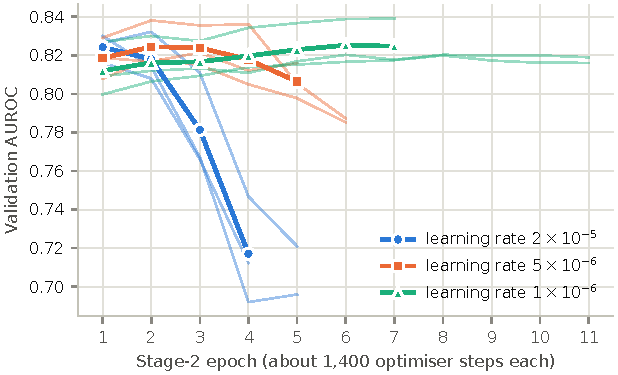
\includegraphics[width=0.62\textwidth]{figures/fig_stage2}
\caption{Validation AUROC during stage-2 fine-tuning for three learning rates. Thin lines are seeds, thick lines their mean over the epochs all three completed.}
\label{fig:stage2}
\end{figure}

\begin{table}
\caption{Effect of the stage-2 learning rate on configuration B0 (three seeds, mean $\pm$ standard deviation). The ensemble column is the score of the average of the three models. Epochs are counted from one.}
\centering
\small
\begin{tabular}{l c c c c c c}
\hline
Stage-2 & \multicolumn{2}{c}{Pooled (A)} & \multicolumn{3}{c}{Within 7.34 s (S7)} & Best stage-2 \\
learning rate & TPR@5\% & AUROC & TPR@5\% & AUROC & Ensemble TPR@5\% & epoch \\
\hline
$2\times10^{-5}$ & $0.436 \pm 0.010$ & 0.829 & $0.384 \pm 0.017$ & 0.787 & 0.404 & 1.7 \\
$5\times10^{-6}$ & $0.423 \pm 0.002$ & 0.834 & $0.381 \pm 0.006$ & 0.792 & 0.396 & 2.7 \\
$1\times10^{-6}$ & $0.404 \pm 0.004$ & 0.830 & $0.362 \pm 0.008$ & 0.784 & 0.375 & 6.7 \\
\hline
\end{tabular}

\label{tab:lr}
\end{table}

\section{Learned layer weights}
With ECG-FM frozen, the head put most of its weight on layers 5 to 9 and least on the last layer (figure \ref{fig:layers}). In step 0, layer \layerFrozenMaxIdx{} received \layerFrozenMax{} of the weight and layer 12 only \layerFrozenMin, a ratio of \layerFrozenRatio. \citet{nguyen2025mol} found middle layers better than the last in a different ECG transformer, and the checkpoint we used had been fine-tuned end to end on the MIMIC-IV-ECG labels, which may bend the last layer towards those labels. Across all \layerFtN{} two-stage checkpoints the largest weight lay between \layerFtMaxLo{} and \layerFtMaxHi{} and the smallest, on layer 12 in \layerFtArgminTwelve{} of them, between \layerFtMinLo{} and \layerFtMinHi. The shape was the same for 10 s inputs and 5 s windows, and the three members of the entry differed by at most \layerEntryRange{} on any layer. The weights start from uniform and received far fewer optimiser steps in two-stage training than in step 0, and the runs that spent longest in stage 2 moved furthest from uniform, so the flat profile may be an artefact of a short stage 2.

\begin{figure}
\centering
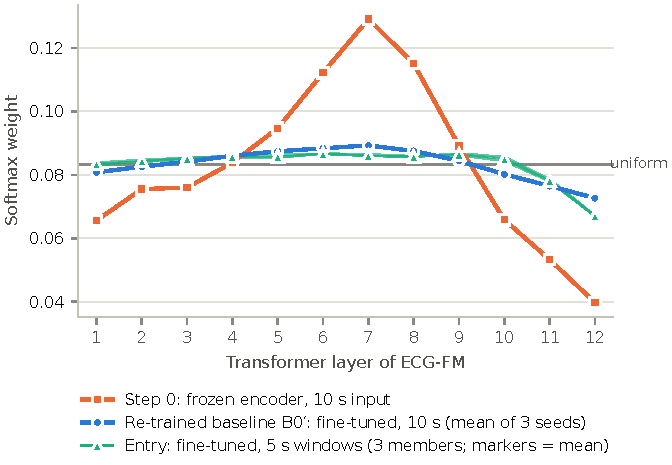
\includegraphics[width=0.62\textwidth]{figures/fig_layers}
\caption{Learned softmax weights over the 12 transformer layers of ECG-FM. Step 0 uses a frozen encoder; the re-trained baseline \Bp{} (mean of three seeds) and the entry's three members are fine-tuned. The horizontal line is the uniform weight, 1/12.}
\label{fig:layers}
\end{figure}

\section{Rounds 2 and 3 in full}
Table \ref{tab:round2} and figure \ref{fig:round2} give every configuration of round 2; the main text keeps the rows of the interpolation comparison. The Challenge score on S10+ did not change significantly (\bzStenPlus{} for B0, \mwStenPlus{} with both remedies). The remedies may also have made the seeds agree: the standard deviation of the S7 \tpr{} across seeds was \bzSsevenSd{} for B0, \mOneSsevenSd{} with matched negatives and \wOneSsevenSd{} with fixed windows, although three seeds give a poor estimate of spread. Figure \ref{fig:round3} shows round 3 seed by seed, laid out as figure \ref{fig:round2}.

\begin{table}
\caption{Round 2 (three seeds each). Differences from the B0 mean, with the SE of a paired bootstrap over test records. The pooled score is \tpr{} on view A.}
\centering
\resizebox{\textwidth}{!}{\begin{tabular}{l c c c c c c c c}
\hline
 & Pooled & \multicolumn{4}{c}{Within 7.34 s records (S7)} & \multicolumn{2}{c}{10 s format (S10+)} & Length- \\
Configuration & TPR@5\% & TPR@5\% & $\Delta$ & AUROC & $\Delta$ & AUROC & $\Delta$ & cue gap \\
\hline
Baseline (B0) & 0.436 & 0.384 & -- & 0.787 & -- & 0.779 & -- & $+0.17$ \\
+ matched negatives (M1) & 0.401 & 0.382 & $-0.002 \pm 0.005$ & 0.786 & $-0.001 \pm 0.003$ & 0.817 & $+0.037 \pm 0.009$ & $+0.04$ \\
+ 5 s windows (W1) & 0.428 & 0.380 & $-0.004 \pm 0.004$ & 0.795 & $+0.008 \pm 0.002$ & 0.835 & $+0.056 \pm 0.010$ & $+0.10$ \\
+ both, fine-tuned ($\alpha=1$) & 0.403 & 0.375 & $-0.009 \pm 0.005$ & 0.795 & $+0.008 \pm 0.003$ & 0.841 & $+0.062 \pm 0.011$ & $+0.01$ \\
+ both, $\alpha=0.5$ & 0.383 & 0.370 & $-0.014 \pm 0.007$ & 0.798 & $+0.011 \pm 0.004$ & 0.833 & $+0.054 \pm 0.012$ & $+0.01$ \\
+ both, frozen ($\alpha=0$) & 0.354 & 0.343 & $-0.041 \pm 0.009$ & 0.775 & $-0.012 \pm 0.006$ & 0.797 & $+0.017 \pm 0.017$ & $+0.00$ \\
\hline
\end{tabular}
}
\label{tab:round2}
\end{table}

\begin{figure}
\centering
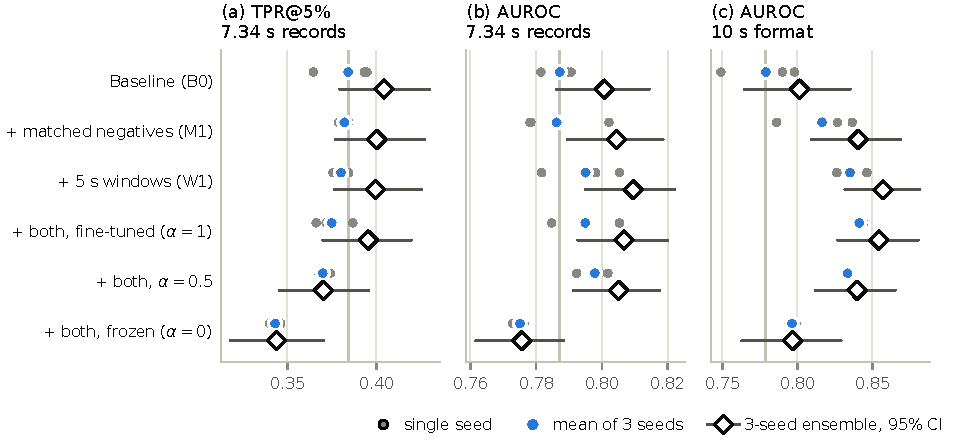
\includegraphics[width=\textwidth]{figures/fig_round2}
\caption{Removing the length cue (round 2; three seeds per row). The vertical line marks the B0 mean. (a) and (b) use held-out CODE-15\% records of 7.34 s; (c) uses the 10 s format (S10+).}
\label{fig:round2}
\end{figure}

\begin{figure}
\centering
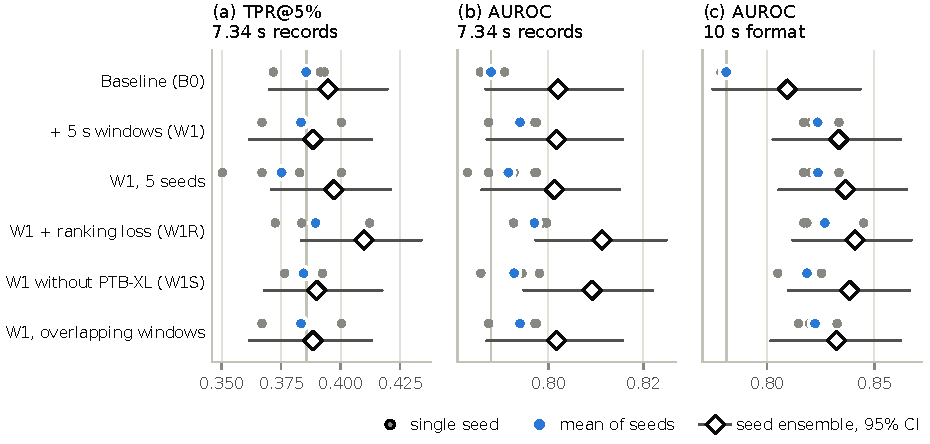
\includegraphics[width=\textwidth]{figures/fig_round3}
\caption{Round 3 under the fixed validation protocol, laid out as figure \ref{fig:round2}; the vertical line marks the \Bp{} mean, and one row has five seeds.}
\label{fig:round3}
\end{figure}

\section{The ablation by length group}
Scoring within one length group lowered the AUROC of every ladder step by a similar amount (figure \ref{fig:inflation}). For B0 it was \bzBauc{} on view B, \bzSsevenAuc{} within 7.34 s records and \bzStenAuc{} within 10.24 s records; with \nStenPos{} positives the last interval is too wide to rank models. For step 0 the pooled AUROC on CODE-15\% records exceeded the within-short AUROC by \rowZeroInflBAuc; the main text uses this difference as the size of what the length cue added.

\begin{figure}
\centering
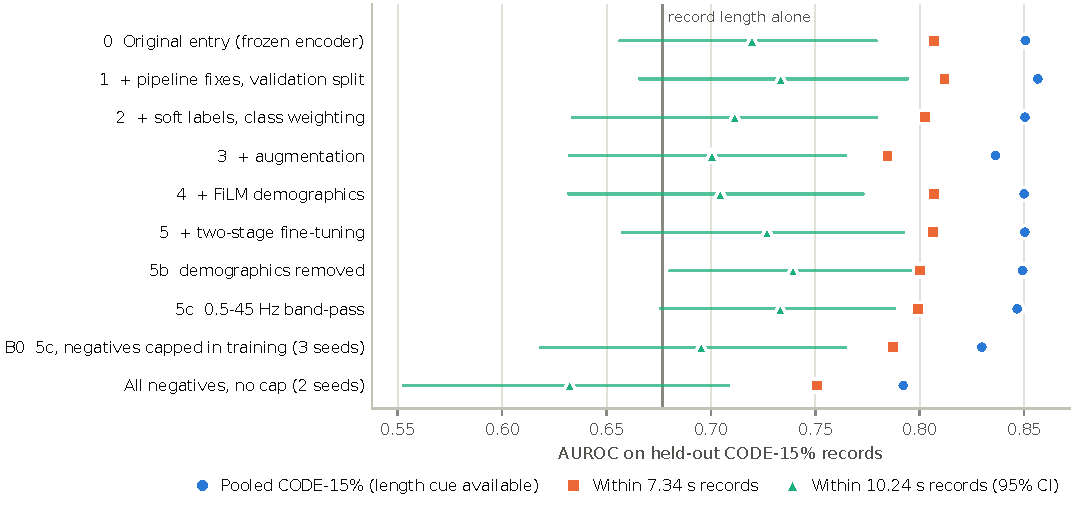
\includegraphics[width=0.95\textwidth]{figures/fig_inflation}
\caption{AUROC of each ablation step on held-out CODE-15\% records: pooled (view B), within 7.34 s records (S7) and within 10.24 s records (S10, with 95\% bootstrap intervals). The vertical line is the AUROC of record length alone on view B.}
\label{fig:inflation}
\end{figure}

\section{Reconstruction and timing}
\textit{Step 0 and the shipped entry.} Step 0 re-creates our Challenge entry in the new code, but it is not the shipped model, and its scores may differ somewhat from those of the entry we submitted in 2025. It resamples with a polyphase filter instead of in the frequency domain (all our runs do), and it trains on 90\% of the training patients, where the shipped model was trained on all of them and saved after the 16th epoch.

\textit{The entry's validation set.} The PTB-XL metadata table that groups records by patient is not part of the Challenge data, so the entry, run as the organisers run it, groups PTB-XL records individually; its validation set has \entryValN{} records instead of the \rThreeValN{} of the round-3 runs. This changes which negatives are held out but no label.

\textit{Time and memory.} The three members of the entry trained in \entryTrainHours{} h on a Titan RTX with a 14.5 GiB memory cap, a projected \entryTfourHours{} h on the organisers' T4 if it is 2.5 times slower, against the 72 h limit. Inference over 2 $\times$ \nTest{} records (the unperturbed and perturbed held-out sets) took \entryInferHours{} h. Fixed 5 s windows cut the peak stage-2 memory from \memTenGiB{} to \memFiveGiB{} GiB.

\section{Views B and C}
\textit{View B} is the held-out CODE-15\% records of every length. It removes the source cue but not the length cue: record length alone reaches an AUROC of \durOnlyB{} there, and \durOnlyA{} on view A. \textit{View C} is view A after perturbations of the kind the organisers applied to the hidden data \citep{reyna2025}: resampling to and from 300--1000 Hz, device-like filtering, noise, baseline wander and mains interference. Once the comparison was made within length groups the perturbations had little effect: \tpr{} within short records was \bzSsevenC{} for B0 and \mwSsevenC{} for the combined configuration on the perturbed records, close to the unperturbed values.

\bibliographystyle{plainnat}
\bibliography{refs}
\end{document}
